\chapter{Analytical Tools For SU(\texorpdfstring{$N$}{N})} \label{apxA}

The analytic computations contained herein revolve around various SU($N$)
dependent quantities, and we therefore need a basis for computing these. In this
appendix we look at how to compute all the necessary components such as the Haar
measure in \secref{sec:haar_measure}, the character integrals in
\secref{sec:character_integrals}, integrals over group polynomials in
\secref{sec:sun_integrals} and finally the fermionic functions of the effective
theory in
\secrefs{sec:evaluating-fermion-determinants,sec:evaluating-polyakov-coupling-terms}.

\section{Computing the Haar measure} \label{sec:haar_measure}

Our first goal is to obtain the invariant group measure of a group element
expressed in terms of its spectral decomposition. Any matrix representation of
an U($N$) matrix has unitary eigenvalues $\lambda_i = e^{i\theta_i}$ only, where
$\sum_i \theta_i = 0 \bmod 2\pi$ for the elements of SU($N$). We write a matrix
$U$ that is a representation of U($N$) in its decomposed form
%
\begin{equation}
  U = W \Lambda W^{\dagger},
\end{equation}
%
where $\Lambda = \diag (e^{i\theta_1}, ..., e^{i\theta_n})$, and $W W^{\dagger}
= \mathbb{1}_R$.  A change in $U$ is therefore
%
\begin{equation}
  \mathrm{d}U = W \mathrm{d} \Lambda W^{\dagger} +  W \big[ W^{\dagger} \mathrm{d}
  W, \Lambda \big] W^{\dagger}.
\end{equation}
%
Using the standard unitary matrix metric, $||M||^2 = \tr(M^{\dagger} M)$,
the size of an infinitesimal square in this coordinate space is
%
\begin{equation} \label{eq:infinitesimal-group-square}
  \mathrm{d} s^2 = \tr (\mathrm{d} U^{\dagger} \mathrm{d} U)
  = \sum_i \mathrm{d} \theta_i^2 + 2 \sum_{i > j}
    \big|e^{i \theta_i} - e^{i\theta_j}\big|^2
    \big| (W^{\dagger} \mathrm{d} W)_{ij} \big|^2 .
\end{equation}
%
Since one identifies the set of coordinates to the metric through
$\mathrm{d} s^2 = g_{\mu\nu} \mathrm{d} \xi^{\mu} \mathrm{d} \xi^{\nu}$,
it is natural to construct the measure as
%
\begin{equation} \label{eq:natural-group-measure}
  \mathrm{d} U(x) = \sqrt{\det g(x)} \prod_{\mu} \mathrm{d}\xi^{\mu}.
\end{equation}
%
To reconcile these two formulae we use the Baker-Campbell-Hausdorff formula to
express $W^{\dagger} \mathrm{d} W$ in terms of the generators of U($d_R$)
%
\begin{equation}
  (W^{\dagger} \mathrm{d} W)_{ij} = i (T_a)_{ij} f_{a b}(w) \mathrm{d} w_b
  \equiv Q_{ijk}(w) \mathrm{d} w_k
\end{equation}
%
with $f$ being some function of the parameters of the generator decomposition.
The general coordinates will thus be a combination of the eigenvalue angles
$\theta_i$ and the parameters $w_i$. The determinant of the metric factorise
into parts dependent on these coordinates, and we get
%
\begin{equation}
  \det g(x) \sim \big(\det Q(w)\big)^2 \prod_{i>j} \big|e^{i\theta_i} -
  e^{i\theta_j}\big|^4.
\end{equation}
%
Since we are concerned with the integrals over the eigenvalues only, one
can integrate out the $w_i$, and get the invariant measure
%
\begin{equation}
  \mathrm{d} U = 
  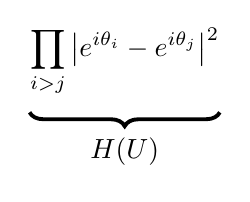
\begin{tikzpicture}[baseline={(trace.base)}]
    \node[inner sep=0pt] (trace) {%
      $\displaystyle\prod_{i>j} \big| e^{i\theta_i} - e^{i\theta_j} \big|^2$};
    \draw [
      decorate,
      line width=1.4pt,
      decoration={
        brace,
        mirror,
        amplitude=5pt
      },
    ]
      ([yshift=-.2cm]trace.south west) -- ([yshift=-.2cm]trace.south east)
      node[midway,below=5pt] {$H(U)$};
  \end{tikzpicture}
  \prod_i \mathrm{d} \theta_i,
\end{equation}
%
where we have identified the Haar measure, $H(U)$. Although this relation is
only true for U($N$), it can be trivially extended to SU($N$) through the
previously mentioned restriction, $\sum_i \theta_i = 0 \bmod 2\pi$.

The \emph{Vandermonde determinant} is introduced to facilitate the calculation
of the Haar measure
%
\begin{equation}
  \prod_{i>j} (z_i - z_j) = \det \mathcal{M} =
  \begin{vmatrix}
    1 & z_1 & \cdots & z_1^{N-1} \\
    1 & z_2 & \cdots & z_2^{N-1} \\
    \vdots & \vdots & \ddots & \vdots \\
    1 & z_N & \cdots & z_N^{N-1} 
  \end{vmatrix},
\end{equation}
%
which can be used to rewrite the Haar measure
%
\begin{equation}
  H(U) = \prod_{i>j} \big| z_i - z_j \big|^2
   = \det \mathcal{M}^{\dagger} \mathcal{M} = \scalemath{0.8}{%
  \begin{vmatrix}
    N & \sum_i z_i & \sum_i z_i^2 & \cdots & \sum_i z_i^{N-1} \\
    \sum_i z_i^{\dagger} & N & \sum_i z_i & \cdots & \sum_i z_i^{N-2} \\
    \vdots & \vdots & \vdots & \ddots & \vdots \\
    \sum_i z_i^{\dagger N-1} & \sum_i z_i^{\dagger N-2} & \sum_i z_i^{\dagger N-3} & \cdots & N
  \end{vmatrix}}.
\end{equation}
%
The fundamental representation of SU($N$) has $N - 1$ independent eigenvalues.
We know that
%
\begin{equation}
  \sum_i z_i^m = \tr U^m \equiv \chi_m,
\end{equation}
%
correspond to the $m$'th powered character. One can therefore use the
Cayley-Hamilton theorem to determine how these angles depend on each other.
The Cayley-Hamilton equation reads
%
\begin{equation} \label{eq:caylay-hamilton}
  M^N + c_{N-1} M^{N-1} + \cdots + c_1 M + (-1)^N \det M\: \mathbb{1}_R = 0,
\end{equation}
%
where the coefficients can be computed recursively using the \emph{Faddeev-LeVerrier
algorithm}
%
\begin{equation}
  c_{N-m} = -\frac{1}{m} \sum_{k=1}^m c_{N-m+k} \tr (M^k).
\end{equation}
%
The first and last coefficient are $c_N = 1$ and $c_1 = (-1)^N \det M$, as can
be inferred from \meqref{eq:caylay-hamilton}.

Using the defining properties of SU($N$), $\det U = 1$ and $U^{\dagger} U =
\mathbb{1}$, we can multiply \meqref{eq:caylay-hamilton} with powers of
$U^{\dagger}$ and trace the equation to find relations between the different
fundamental characters, and thus reduce the number of unknowns in the Haar
measure.

For instance, for SU($3$), $\chi_2 = \chi^2 - 2 \chi^*$, giving
%
\begin{equation} \label{eq:su3-haar-measure}
  H(U) =
  \begin{vmatrix}
    3 & \chi & \chi^2 - 2 \chi^* \\
    \chi^* & 3 & \chi \\
    \chi^{*2} - 2 \chi & \chi^* & 3
  \end{vmatrix} = 27 - 18\, |\chi|^2  + 8 \mathrm{Re}\, \chi^3 - |\chi|^4.
\end{equation}

\section{\texorpdfstring{$\chi_r \chi_s$}{Ln Lm} integrals} \label{sec:character_integrals}

A specific set of integrals we encounter often are integrals of the form
%
\begin{equation} \label{eq:character_integral_before}
  I_{nm} = \int \mathrm{d} U \, \chi(U)^n \chi(U^{\dagger})^m.
\end{equation}
%
These can be most easily calculated through their trigonometric decomposition.
Using
%
\begin{equation}
  \begin{tikzpicture}[baseline={([yshift=-.55ex] aligned.center)}]
    \node (aligned) {%
      $\begin{aligned}
        \chi(U) &= {\textstyle\sum_{\alpha=1}^N} e^{i \theta_\alpha} \\
        \chi(U^{\dagger}) &= {\textstyle\sum_{\alpha=1}^N} e^{- i \theta_\alpha}
      \end{aligned}$};
    \draw [
      decorate, line width=1.4pt,
      decoration={ brace, mirror, amplitude=5pt },
    ] (aligned.south east) -- (aligned.north east);
  \end{tikzpicture}
  \hskip1em {\textstyle\sum_{\alpha=1}^N} \theta_{\alpha} = 0 \bmod 2\pi,
\end{equation}
%
\meqref{eq:character_integral_before} yields
%
\begin{equation}
  I_{nm} = \int \big[ \mathrm{d} \theta \big]_i\, H(U)
  \delta\big({\textstyle\sum}\theta_i = 0\big)
  \sum_{\{n_i\}} \sum_{\{m_i\}} \prod_{k=1}^n
  \prod_{l=1}^m \frac{k l}{n_k! m_l!} e^{i n_k \theta_k - i m_l \theta_l} \,,
\end{equation}
%
with sums over integer partitions so that
%
\begin{equation}
  \sum_{i=1}^N (n,m)_i = (n,m).
\end{equation}
%
As the pure phase integrals give
%
\begin{equation} \label{eq:oscillating-integral}
  \int_{\mathrlap{-\pi}}^{\pi} \mathrm{d}\alpha \, e^{in \alpha} = \delta(n),
  \text{ for } n \in \mathbb{Z} \,,
\end{equation}
%
only combinations where the exponential's arguments cancel will give a non-zero
contribution, and calculating the integral reduces to finding these combinations.

\subsection{Integrals over characters of SU\texorpdfstring{($3$)}{(3)}}

As this is not a problem that is solvable in general, we specialise to the group
SU($3$). In this case we only have two free angles, which we label $\theta$ and
$\phi$. The full integral is
%
\begin{align}
  &I_{nm} = \int \mathrm{d} \theta \mathrm{d} \phi \, H(\theta,\phi)
  \big(e^{i\theta} + e^{i\phi} + e^{-i(\theta + \phi)}\big)^n
  \big(e^{-i\theta} + e^{-i\phi} + e^{i(\theta + \phi)}\big)^m \nonumber\\
  &=\int \mathrm{d} \theta \mathrm{d} \phi \, H(\theta,\phi)
  \sum_{\{l_i\}} \sum_{\{k_i\}} \frac{n!}{l_1! l_2! l_3!} \frac{m!}{k_1! k_2!
    k_3!} e^{i \theta (l_1 - l_3 - k_1 + k_3) + i \phi (l_2 - l_3 - k_2 + k_3)}.
\end{align}
%
We define the measure-less integral $J_{nm} = \int [\mathrm{d} \theta]_i\,
\chi^n \chi^{*m}$, which is
%
\begin{equation}
  J_{nm} = (2\pi)^2 \sum_{\{l_i\}} \sum_{\{k_i\}}
    \frac{n!}{l_1! l_2! l_3!} \frac{m!}{k_1! k_2!k_3!}\,
    \delta\big(l_1 - l_3 - k_1 + k_3\big)\, \delta\big(l_2 - l_3 - k_2 + k_3\big).
\end{equation}
%
Carrying out the explicit sums over four variables yields
%
\begin{equation}
  J_{nm} = (2\pi)^2 \sum_{l = 0}^n \sum_{k = 0}^m
    \frac{n!}{l!\, (k + \frac{n-m}{3})!\,(\frac{2n+m}{3} - l - k)!}
    \frac{m!}{k!\, (l + \frac{m-n}{3})!\,(\frac{2m+n}{3} - l - k)!}
\end{equation}
%
where the remaining variables $l$ and $k$ are restricted by the requirement that
the factorials all have non-negative arguments. Since the Haar measure itself is
expressed in terms of the characters, we see from \meqref{eq:su3-haar-measure}
that
%
\begin{equation}
  I_{n,m} = 27\, J_{n,m} - 18\, J_{n+1,m+1} + 4\, J_{n+3,m} + 4\, J_{n,m+3} - J_{n+2,m+2}.
\end{equation}
%
It is easy to see that $J_{nm}$ is symmetric in its indices, $J_{nm} = J_{mn}$,
and by extension, so it $I_{nm}$. We introduce the normalised integral,
$\tilde{I}_{nm} = I_{nm} / I_{00}$, the value of some of which are listed in
\tabref{tab:character-integrals}. Analysing the sequences one notices that they
have deep combinatorial connections \citep{OEIS}. For instance, the first row of
this table is the sequence of permutations of $S_n$ with longest increasing
subsequence length $<=3$ (A005802). The first column of the table on the other
hand corresponds to the 3 dimensional Catalan numbers (A005789). A more thorough
review of the combinatorics of SU($3$) can be found in \citep{Unger:2014oga}.

\begin{table}
  \begin{center}
    \begin{tabular}{*8c} \toprule
      {$\tilde{I}_{nm}$} & $\mathbb{1}$ & $\chi\chi^*$ & $(\chi\chi^*)\mathrlap{^2}$ & $(\chi\chi^*)\mathrlap{^3}$ 
        & $(\chi\chi^*)\mathrlap{^4}$ & $(\chi\chi^*)\mathrlap{^5}$ & $(\chi\chi^*)\mathrlap{^6}$ \\\midrule
      $\mathbb{1}$ & 1 & 1 & 2 & 6 & 23 & 103 & 513 \\
      $\chi^3$ & 1 & 3 & 11 & 47 & 225 & 1\,173 & 6529 \\
      $\chi^6$ & 5 & 21 & 98 & 498 & 2\,709 & 15\,565 & 93\,500 \\
      $\chi^9$ & 42 & 210 & 1\,122 & 6\,336 & 37\,466 & 230\,230 & 1\,461\,330 \\
      $\chi^{12}$ & 462 & 2\,574 & 15\,015 & 91\,091 & 571\,428  & 3\,688\,932 & 24\,410\,334 \\
      $\chi^{15}$ & 6\,006 & 36\,036 & 223\,652 & 1\,429\,428 & 9\,372\,168 & 62\,833\,836 & 429\,568\,036 \\\bottomrule
    \end{tabular}
  \end{center}
  \caption{Some integrals over the characters of SU($3$) where the integrand is made
    up of the product of the topmost row with the leftmost column. All other
    integrals are zero due to the selection rule of
    \protect\meqref{eq:integral-selection-rule}.}
  \label{tab:character-integrals}
\end{table}

\subsection{Characters of plaquettes}

Another set of integrals that appears often, are those of characters over
plaquettes sharing a common link, such as the ones in
\secref{sec:pure-gauge-theory}. These integrals are of the form
%
\begin{equation}
  F_{nm}^r(V,W) = \int \mathrm{d} U \, \chi_r(VU)^n \chi_r(WU^{\dagger})^m.
\end{equation}
%
In \citep{Bars:1979xb} the authors introduced a recursive formula to evaluate
the diagonal integrals of this form in the fundamental representation of U($N$),
namely the integrals $F_{nn}^f(V,V^{\dagger})$. The procedure is as follows. First one
introduces a new integral
%
\begin{equation}
  G_n(\{V_i\}) = \int \mathrm{d} U \> \chi_f(V_1 U) \cdots \chi_f(V_n U) \,
    \chi_f(V_1^{\dagger} U^{\dagger}) \cdots \chi_f(V_n^{\dagger} U^{\dagger}),
\end{equation}
%
and verifies that by using the special form $(A_n)_{kl} = \delta_{ik}
\delta_{lq}$, $(A_n^{\dagger})_{kl} = \delta_{qk} \delta_{lj}$ for some of the
integers $i,j,q$, the final factors of $G$ simplify when summing over $k$
%
\begin{equation}
  {\textstyle\sum_k} G_n(\{V_i\}) = \delta_{ij} G_{n-1}(\{V_i\}').
\end{equation}
%
Due to the properties of the integrand of $G$, it has to be U($N$) $\times$
U($N$) invariant, and we can therefore decompose any $G$ into its invariant
combinations. For instance, the two lowest orders yield
%
\begin{align}
  G_1(A_1) &= \int \mathrm{d} U \> \chi_f(A_1 U) \, \chi_f(A_1^{\dagger} U^{\dagger})
   = C_1 \> \chi_f(A_1 A_1^{\dagger}), \\
  G_2(A_1,A_2) &= \int \mathrm{d} U \> \chi_f(A_1 U) \chi_f(A_2 U) 
  \chi_f(A_1^{\dagger} U^{\dagger}) \chi_f(A_2^{\dagger} U^{\dagger})  \nonumber \\
  &= C_1 \big( \chi_f(A_1 A_1^{\dagger}) \chi_f(A_2 A_2^{\dagger}) + \chi_f(A_1
  A_2^{\dagger}) \chi_f(A_2 A_1^{\dagger})\big) \nonumber \\
  &\hskip2em+ C_2 \big(\chi_f(A_1 A_1^{\dagger} A_2 A_2^{\dagger})
  + \chi_f(A_1 A_2^{\dagger} A_2 A_1^{\dagger}) \big).
\end{align}
%
One then inserts the special form for $A_n$ on the left and right hand side of
the equations and systematically determine the unknown parameters $C_i$.

\section{\texorpdfstring{$g^n (g^{-1})^m$}{Un Udm} integrals} \label{sec:sun_integrals}

In this section we present a method of computing integrals over
matrix representations of the SU($N$) members, namely integrals of the form
\meqref{eq:group-integrals-representation}
%
\begin{equation}
  I_{i_1,j_1,...,i_n,j_n}^{k_1,l_1,...,k_m,l_m} = \int \mathrm{d} U \,
    U_{i_1j_1} \cdots U_{i_nj_n} U^{\dagger}_{k_1l_1} \cdots U^{\dagger}_{k_ml_m}.
\end{equation}
%
Although there are multiple ways to approach this, we will closely follow the
paper of \citeauthor{Creutz:1977yy} [\citeyear{Creutz:1977yy,Creutz:1978ub}].
First we introduce the generating functional
%
\begin{equation}
  \mathcal{W}(J,K) = \int \mathrm{d} U \, \exp \Big( \tr \big(J U + K U^{\dagger}\big) \Big)
\end{equation}
%
noting that we can use it to reexpress $I$
%
\begin{equation}
  I_{i_1,j_1,...,i_n,j_n}^{k_1,l_1,...,k_m,l_m} = \bigg(
    \frac{\delta}{\delta J_{i_1j_1}} \cdots \frac{\delta}{\delta J_{i_nj_n}}
    \frac{\delta}{\delta K_{k_1l_1}} \cdots \frac{\delta}{\delta K_{k_ml_m}}
    \bigg) \mathcal{W}(J,K) \bigg|_{J=K=0}.
\end{equation}
%
We then use the cofactor expansion of $U^{\dagger}$ to remove the dependence on
$K$
%
\begin{align}
  U^{\dagger}_{ij} &= \frac{1}{\det U} \big( \cof U^T \big)_{ij} \nonumber\\
  &= \frac{1}{(N-1)!} \epsilon_{j, i_1, \dots, i_{N-1}} \epsilon_{i, j_1, \dots, j_{N-1}}
    U_{i_1j_1} \cdots U_{i_{N-1}j_{N-1}}.
\end{align}
%
where we have introduced the completely anti-symmetric tensors $\epsilon$.
We factor out the dependence on $K$ of the generating functional
%
\begin{equation}
  \mathcal{W}(J,K) = \exp\bigg( \tr \Big( K \cof \frac{\delta}{\delta J} \Big) \bigg)
  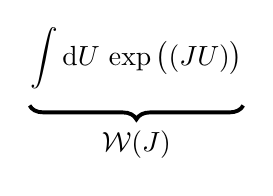
\begin{tikzpicture}[baseline={(trace.base)}]
    \node[inner sep=0pt] (trace) {%
      $\displaystyle\int \mathrm{d} U \, \exp \big( \tr (JU) \big)$};
    \draw [
      decorate,
      line width=1.4pt,
      decoration={
        brace,
        mirror,
        amplitude=5pt
      },
    ]
      ([yshift=-.2cm]trace.south west) -- ([yshift=-.2cm]trace.south east)
      node[midway,below=5pt] {$\mathcal{W}(J)$};
  \end{tikzpicture}\,.
\end{equation}
%
Using a determinant expansion of $\mathcal{W}(J)$, which is allowed due to the fact that
$\mathcal{W}(VUW) = \mathcal{W}(U)$ for arbitrary matrices $W, V \in
\text{SU}(3)$ \citep{Creutz:1977yy}, we finally obtain
%
\begin{equation}
  \mathcal{W}(J) = \sum_{i=0}^{\infty} \frac{2! \cdots (N-1)!}{i! \cdots
    (i+N-1)!} \big(\det J\big)^i.
\end{equation}
%
Although this expression is a little unwieldy, we immediately see a selection
rule for the integrals. Using the fact that the determinant of an $N \times N$ matrix is a
polynomial of $N$'th power of its elements
%
\begin{equation}
  \det M = \frac{1}{N!} \epsilon_{i_1,\dots,i_N} \epsilon_{j_1, \dots, j_N}
  M_{i_1j_1} \cdots M_{i_Nj_N},
\end{equation}
%
only factors of $N$'th power derivatives of $\mathcal{W}$ will
survive when we set $J=0$. Since the cofactor is a $N-1$'th power polynomial we
get the selection rule
%
\begin{equation} \label{eq:integral-selection-rule}
  \int \mathrm{d} U \, U^n U^{\dagger m} \neq 0  \hskip1em\iff\hskip1em n + (N-1)m = 0 \pmod N.
\end{equation}
%
Finally, we compute the most used integral of this thesis
%
\begin{align}
  I_{ij}^{kl} &= \int \mathrm{d} U \, U_{ij} U^{\dagger}_{kl} \nonumber\\
  &= \frac{1}{(N-1)!} \epsilon_{l,i_1,\dots,i_{N-1}} \epsilon_{k, j_1, \dots, j_{N-1}}
    \int \mathrm{d} U \, U_{ij} U_{i_1j_1} \cdots U_{i_{N-1}j_{N-1}} \nonumber\\
  &= \frac{1}{(N-1)!} \epsilon_{l,i_1,\dots,i_{N-1}} \epsilon_{k, j_1, \dots, j_{N-1}}
    \bigg( \frac{\delta}{\delta J_{ij}} \frac{\delta}{\delta J_{i_1j_1}} \cdots
    \frac{\delta}{\delta J_{i_{N-1}j_{N-1}}} \bigg) \mathcal{W}(J) \bigg|_{J=0}
    \nonumber \\
  &= \frac{1}{N!(N-1)!} \epsilon_{l,i_1,\dots,i_{N-1}} \epsilon_{k, j_1, \dots, j_{N-1}}
  \epsilon_{i,i_1,\dots,i_{N-1}} \epsilon_{j,j_1,\dots,j_{N-1}} \nonumber \\
  &= \frac{1}{N!(N-1)!} (N-1)!\,\delta_{il}\,(N-1)!\,\delta_{jk} = \frac{1}{N}
  \delta_{il} \delta_{jk} .
  \label{eq:uub-integral}
\end{align}

\section{Static determinant} \label{sec:evaluating-fermion-determinants}

With the measure and various link integrals at hand, it is time we approach the
two fundamental fermionic quantities of the effective theory, namely the static
determinant and one-site interactive loop terms. The latter we will cover in the
next section, and we will focus on the static determinant here, namely
%
\begin{equation}
  \det Q_{\text{stat}} = \prod_{\vec{x}} \det ( 1 + h_1 W(\vec{x}) )^2 
    \det ( 1 + \bar{h}_1 W^{\dagger}(\vec{x}) )^2.
\end{equation}
%
Since these factors are all independent quantities, we can focus on determining
a single determinant $\det(1 + h_1 W)$, restricting ourselves to $W \in
\text{SU($N$)}$ for the current study. The determinant can be rewritten using the
trace log identity together with the Mercator series, giving
%
\begin{equation}
  \det ( 1 + h_1 W ) = \sum_{n=0}^N \sum_{\{k_i\}_n} \prod_{l=1}^N
  \frac{(-1)^{(l+1)k_l}}{l^{k_l} k_l!} h_1^{l k_l} \tr (W^l)^{k_l},
\end{equation}
%
with indices $\{k_i\}_n$ summed over a range bounded by the equations
%
\begin{equation} \textstyle
  \sum_{i=1}^{N} k_i = n, \hskip1em\text{and}\hskip1em
  \sum_{i=1}^N i k_i \leq N .
\end{equation}
%
The highest power term of the Mercator series is fixed by the fact that $\det W
= 1$, and we can thus reduce it out of the problem using the Cayley-Hamilton
equation \eqref{eq:caylay-hamilton}. The static determinants of groups SU($1 \to
5$) are listed in \tabref{tab:static-determinant}.

\begin{table}
  \begin{center}
    \begin{tabular}{cl} \toprule
      SU($N$) & $\det(1 + h_1 W)$ \\ \midrule
      $1$ & $1 + h_1$ \\
      $2$ & $1 + h_1^2 + h_1 \chi_1$ \\
      $3$ & $1 + h_1^3 + h_1\chi_1 + \frac{1}{2} h_1^2 (\chi_1^2 - \chi_2)$ \\
      $4$ & $1 + h_1^4 + h_1 \chi_1 + \frac{1}{2} h_1^2 (\chi_1^2 - \chi_2) +
      \frac{1}{6} h_1^3 (\chi_1^3 - 3 \chi_1 \chi_2 + 2 \chi_3)$ \\
      \multirow{2}{*}{$5$} & $1 + h_1^5 + h_1 \chi_1 + \frac{1}{2} h_1^2 (\chi_1^2 - \chi_2) +
      \frac{1}{6} h_1^3 (\chi_1^3 - 3 \chi_1 \chi_2 + 2 \chi_3) $ \\
      & $ + \frac{1}{24} h_1^4 ( \chi_1^4 - 6 \chi_1^2 \chi_2 + 3 \chi_2^2 +
      8\chi_1 \chi_3 - 6\chi_4 )$ \\ \bottomrule
    \end{tabular}
  \end{center}
  \caption{Static determinants calculated in various groups SU($N$) with the
    independent characters $\chi_i = \tr(U^i)$.}
  \label{tab:static-determinant}
\end{table}

\section{\texorpdfstring{$W_{nm}$}{Wnm} terms}
\label{sec:evaluating-polyakov-coupling-terms}

The last group dependent quantity of interest is the effective theory nodes,
which have the form
%
\begin{equation}
  W_{nm} = \tr \frac{(h_1 W)^m}{(1 + h_1 W)^n},
\end{equation}
%
and need to be rewritten in terms of the characters. There are multiple ways to
work with these quantities. First of all, they can be studied directly though
their series expansion
%
\begin{equation}
  W_{nm} = \tr \Big( (h_1 W)^m \sum_{k=0}^{\infty} \binom{k + n - 1}{k} (-h_1 W)^k \Big)
\end{equation}
%
which is useful for some particular identities. Alternately one can rewrite it in
terms of its independent factors
%
\begin{equation}
  W_{nm} = \sum_{i=0}^{N-1} a_i \tr{W^i},
\end{equation}
%
then use a combination of its series expansion and the Cayley-Hamilton theorem
to manipulate the expression and solve for $a_i$. Finally, one can construct a
generating functional to convert between the different variables. One such
functional can conveniently be constructed using the expression for the static
determinant
%
\begin{equation}
  G(\alpha,\beta) = \log \det ( \alpha + \beta h_1 W ),
\end{equation}
%
from which
%
\begin{equation}
  W_{nm} = \frac{(-1)^{n-1}}{(n-1)!} \frac{\partial^{(n-m)}}{\partial \alpha^{(n-m)}}
    \frac{\partial^{m}}{\partial \beta^m} G(\alpha,\beta)
    \bigg|_{\alpha=\beta=1}.
\end{equation}
%
The generating functional can in turn be calculated with the methods outlined in
the previous sections.
